% ============================================================================
\section{Results}
\label{sec:results}
% ============================================================================
% FIRST DRAFT, written 2026-10-13 from scripts 04 to 08. Every number below is
% printed by the script named next to it; rerun the script before trusting a
% number here.

\subsection{Pair production from the bare vacuum}

Figure~\ref{fig:pairs} shows the particle density after a quench from the bare
vacuum, computed exactly. Energy is conserved to \num{4e-15} throughout and the
total charge never leaves zero. Nothing is injected: the bare vacuum is not an
eigenstate of the full Hamiltonian, and the energy it already holds moves between
the electric field and the rest mass of the pairs. Table~\ref{tab:quench} makes
this quantitative. The larger the gap between the energy of the bare vacuum and
the true ground-state energy, the more pairs appear, and the relation is
monotone across the four masses studied. The two outer links carry identical
flux at every time, $|\langle\Lop{1}\rangle - \langle\Lop{3}\rangle| <
\num{1e-15}$, as the CP symmetry of Eq.~\eqref{eq:cp} requires.

\begin{figure}[t]
  \centering
  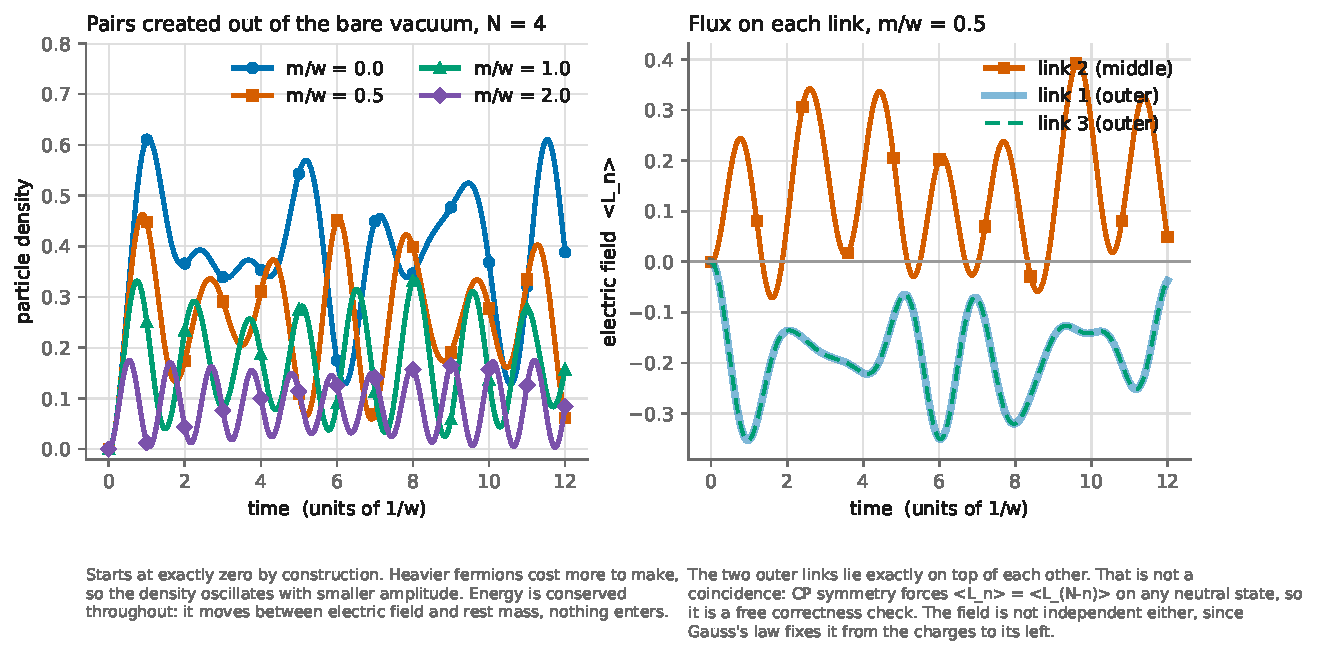
\includegraphics[width=\textwidth]{04_pair_production.pdf}
  \caption{Left: particle density against time after a quench from the bare
  vacuum, for four fermion masses, computed exactly. Right: the electric field
  on each link at $m = 0.5\,w$; the two outer links coincide, as CP requires.
  Produced by \texttt{scripts/04\_pair\_production\_preview.py}.}
  \label{fig:pairs}
\end{figure}

\begin{table}[t]
  \centering
  \caption{Why pairs appear. $E_{\mathrm{bare}}$ is the energy of the bare
  vacuum, $E_0$ the exact ground-state energy, and $\nu_{\max}$ the largest
  particle density reached for $0 \le t \le 12$ ($J = w$).}
  \label{tab:quench}
  \small
  \begin{tabular}{ccccc}
    \toprule
    $m/w$ & $E_{\mathrm{bare}}$ & $E_0$ & $E_{\mathrm{bare}} - E_0$ & $\nu_{\max}$ \\
    \midrule
    0.0 & $\phantom{-}0.000$ & $-1.477$ & 1.477 & 0.612 \\
    0.5 & $-1.000$ & $-2.075$ & 1.075 & 0.463 \\
    1.0 & $-2.000$ & $-2.828$ & 0.828 & 0.335 \\
    2.0 & $-4.000$ & $-4.553$ & 0.553 & 0.175 \\
    \bottomrule
  \end{tabular}
\end{table}

\subsection{Trotter error against shot noise: the crossover}

The Trotter error scales with the predicted exponents (Figure~\ref{fig:trotter},
left), so its size at any step can be trusted. Figure~\ref{fig:trotter} (right)
compares the Trotter bias in the particle density at $t = 3$ with the shot-noise
uncertainty. The standard error is \num{0.0176} at 256 shots and \num{0.0047} at
4096, and the Trotter bias falls below these floors at $\delta t \approx 0.19$
and $\delta t \approx 0.094$ respectively. At the first recombination minimum,
$t = 1.76$, the crossover sits at $\delta t = 0.44$, $0.35$ and $0.22$ for 256,
1000 and 4096 shots (\texttt{scripts/08}). Below the crossover a smaller step
buys accuracy the statistics cannot resolve, while the circuit keeps growing:
the two-qubit gate count at $t = 3$ rises from 320 at $\delta t = 0.3$ to 6400
at $\delta t = 0.015$.

\begin{figure}[t]
  \centering
  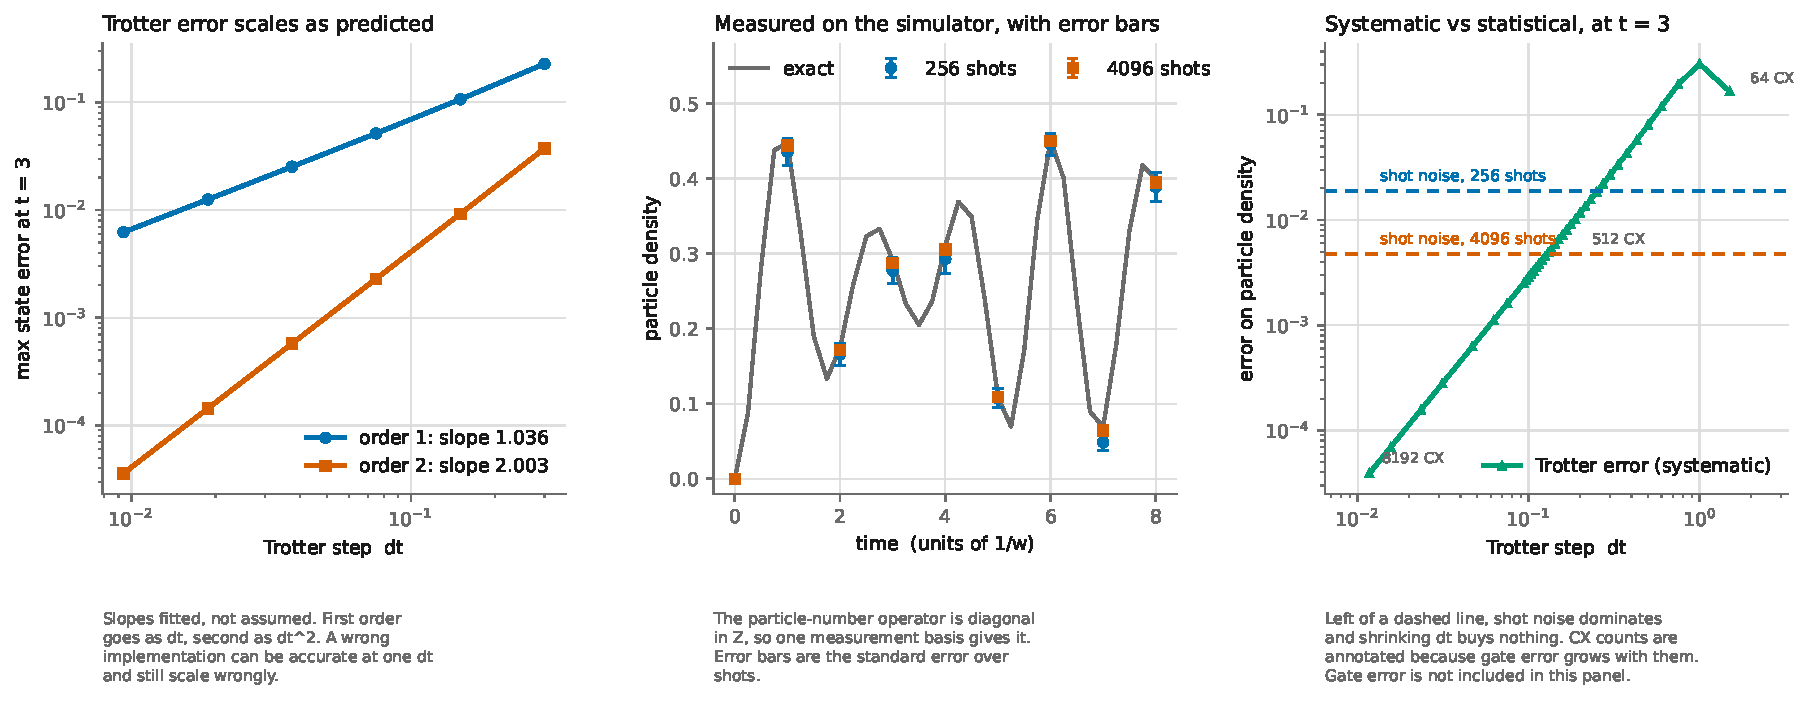
\includegraphics[width=\textwidth]{05_qiskit_trotter.pdf}
  \caption{Left: Trotter error against step size, with the scaling exponent
  fitted rather than assumed. Centre: particle density measured from finite
  shots. Right: the crossover between Trotter bias and shot noise at $t = 3$.
  Produced by \texttt{scripts/05\_qiskit\_trotter.py}.}
  \label{fig:trotter}
\end{figure}

\subsection{Gate error and the failure threshold}

Figure~\ref{fig:threshold}(a) shows what depolarising gate error does to the
pair-production signal at $\delta t = 0.1$. The density is pulled toward the
maximally mixed value $\tfrac12$, the later times first, because their circuits
are deeper. At $\epsilon_2 = 10^{-3}$ the recombination dip keeps about half its
noiseless size; at $\epsilon_2 = 10^{-2}$ it is gone.
Figure~\ref{fig:threshold}(b) and Table~\ref{tab:threshold} give the failure
threshold for three step sizes.

\begin{table}[t]
  \centering
  \caption{Failure threshold $\epsilon^\ast$, the two-qubit error at which the
  recombination dip falls to twice its shot-noise uncertainty, with
  $\epsilon_1 = \epsilon_2/10$. $n_{\mathrm{CX}}$ is the CX count of the deeper
  (trough) circuit. From \texttt{scripts/06\_noise\_threshold.py}.}
  \label{tab:threshold}
  \small
  \begin{tabular}{cccccc}
    \toprule
    $\delta t$ & $n_{\mathrm{CX}}$ & $\epsilon^\ast$ ($10^3$ shots) & $\epsilon^\ast n_{\mathrm{CX}}$
      & $\epsilon^\ast$ ($10^4$ shots) & $\epsilon^\ast$ (no shot noise) \\
    \midrule
    0.1 & 576 & \num{3.3e-3} & 1.92 & \num{4.0e-3} & \num{4.6e-3} \\
    0.2 & 288 & \num{6.9e-3} & 1.98 & \num{8.4e-3} & \num{9.4e-3} \\
    0.3 & 192 & \num{1.06e-2} & 2.03 & \num{1.29e-2} & \num{1.45e-2} \\
    \bottomrule
  \end{tabular}
\end{table}

The threshold is set by circuit depth. At 1000 shots the product
$\epsilon^\ast n_{\mathrm{CX}}$ lies between 1.92 and 2.03 for all three step
sizes: the signal is lost once the deepest circuit has accumulated about two
two-qubit errors on average. This follows from the dip itself. Under depolarising
noise $D$ shrinks roughly in proportion to the fidelity $F$ of the trough
circuit, so the signal disappears when $F$ falls to $2\sigma_D/D_0 \approx 0.07$,
and with $F \approx e^{-c\,\epsilon_2 n_{\mathrm{CX}}}$ that fixes the product
$\epsilon_2 n_{\mathrm{CX}}$. More shots buy little. Going from $10^3$ to $10^4$
shots raises the threshold by only about 20\,\%, because $F$ falls exponentially
with gate count while the noise floor falls only as $M^{-1/2}$.
\todo{Compare with the two-qubit fidelity of 99.6\,\% quoted by Rosanowski
\emph{et al.}\ and with the gate counts of Martinez \emph{et al.}\ and Farrell
\emph{et al.}}

\begin{figure}[t]
  \centering
  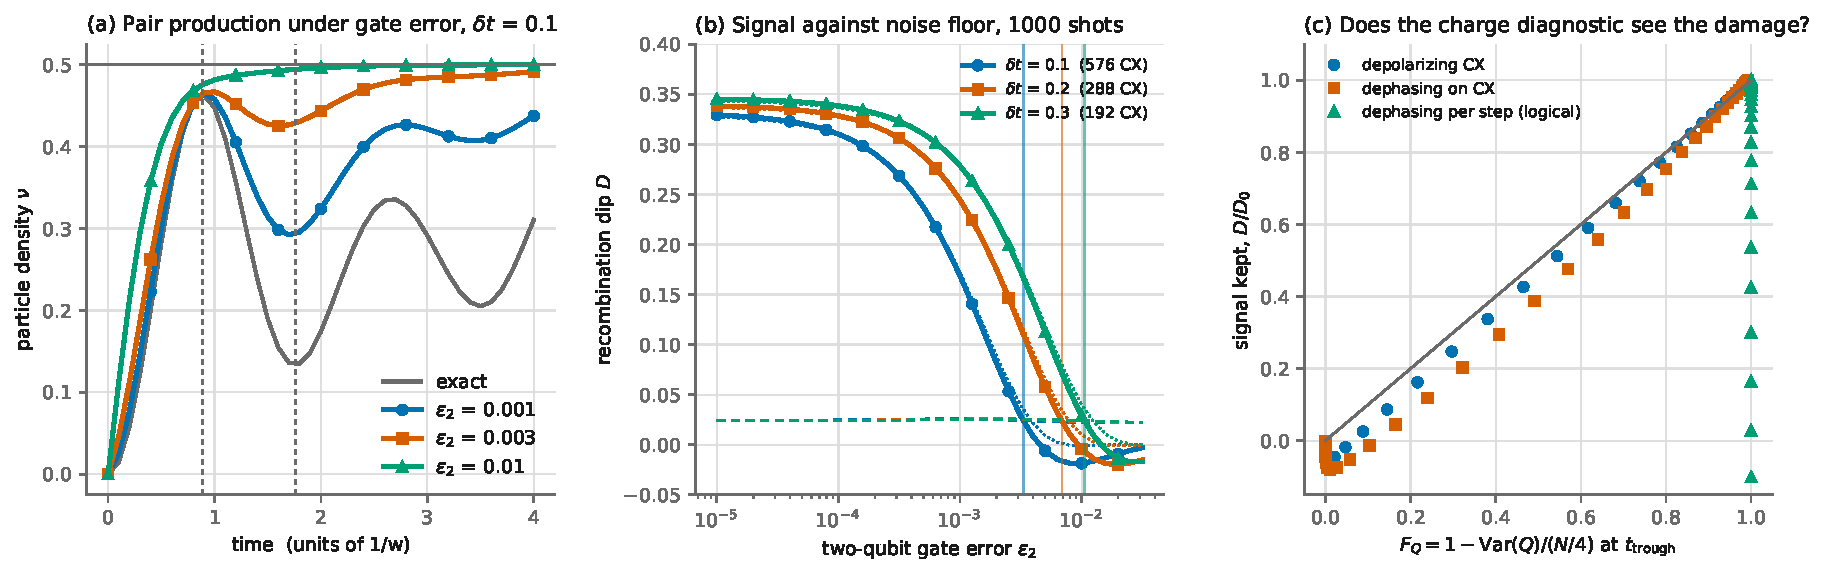
\includegraphics[width=\textwidth]{06_noise_threshold.pdf}
  \caption{(a) Particle density under depolarising gate error at
  $\delta t = 0.1$; dashed lines mark $t_{\mathrm{p}}$ and $t_{\mathrm{t}}$.
  (b) Recombination dip $D$ (solid), twice its shot-noise uncertainty at 1000
  shots (dashed), and the dip predicted from charge-conservation data taken at
  $\epsilon_0 \approx \epsilon^\ast/10$ (dotted). Vertical lines mark
  $\epsilon^\ast$. (c) Signal retained against the fidelity read from
  $\mathrm{Var}(Q)$, Eq.~\eqref{eq:FQ}; the diagonal is perfect prediction.
  Produced by \texttt{scripts/06\_noise\_threshold.py}.}
  \label{fig:threshold}
\end{figure}

\subsection{Does charge conservation predict the threshold?}

For gate noise it does, to within about 15\,\%, and it errs in one direction.
Using only the charge variance measured at one noise level
$\epsilon_0 \approx \epsilon^\ast/10$, the procedure of
Section~\ref{sec:budget-method} predicts thresholds 1.15, 1.14 and 1.17 times
the true value for $\delta t = 0.1$, $0.2$ and $0.3$ at 1000 shots, and 1.10 to
1.13 times it from $\epsilon_0 \approx \epsilon^\ast/3$. The prediction is always
optimistic: real gate noise erodes the dip somewhat faster than a global
depolarising channel with the same charge violation would.
Figure~\ref{fig:threshold}(c) shows why. The points for depolarising and for
gate-level dephasing noise lie close to the diagonal but slightly below it. At
$10^4$ shots the threshold sits at lower fidelity, where this small offset
matters more, and the overestimate grows to between 19 and 36\,\%.

For dephasing on the logical state the diagnostic fails completely.
$\mathrm{Var}(Q)$ stays at \num{1e-33} while the dip shrinks to zero at a
phase-flip probability of 0.036 per qubit per step, and the points in
Figure~\ref{fig:threshold}(c) form a vertical line at $F_Q = 1$. The CP
asymmetry is equally blind, because a uniform dephasing channel respects CP. A
charge-based diagnostic therefore bounds the damage from errors that move charge
and says nothing about errors that only scramble phases. This matters for the
literature: the error model Martinez \emph{et al.}\ fitted to their four-qubit
data was exactly this kind of dephasing~\cite{martinez2016}.
\todo{Discuss against Nguyen et al.\ symmetry protection, which targets coherent
errors, and Halimeh and Hauke on the slow growth of gauge violation.}

\subsection{The full budget and the optimal step size}

Figure~\ref{fig:budget}(a) puts all four sources together for one 1000-shot
measurement of $\nu(t_{\mathrm{t}})$ with 1\,\% readout error. Without gate
error the total error falls as $\delta t$ shrinks until it reaches the floor set
by shot noise and readout bias. With gate error it has a minimum. The optimal
step is $\delta t = 0.35$ (160 CX) at $\epsilon_2 = 3\times 10^{-4}$,
$0.44$ (128 CX) at $10^{-3}$, and $0.59$ (96 CX) at $3\times10^{-3}$: the worse
the hardware, the coarser the best Trotter step. At the optimum gate error
dominates, and the Trotter bias is between a quarter and two-fifths of it.
Refining the step past the optimum makes the answer worse, as the proposal
anticipated, and the figure shows by how much.

The decomposition depends on the observable (Figure~\ref{fig:budget}(b)). At
$\epsilon_2 = 10^{-3}$ and the optimal step, gate error is 89\,\% of the summed
squared error on the particle density, 59\,\% on the outer-link field, and only
29\,\% on the middle-link field, where Trotter error dominates. The middle-link
field is nearly immune to depolarising noise because its exact value at this
time, $-0.05$, is already close to its value in the maximally mixed state, zero;
the outer links sit at $-0.16$, far from their mixed-state value of $-0.5$. An
observable whose ideal value lies near its mixed-state value has little left for
depolarising noise to erase, and correspondingly little signal.

\begin{figure}[t]
  \centering
  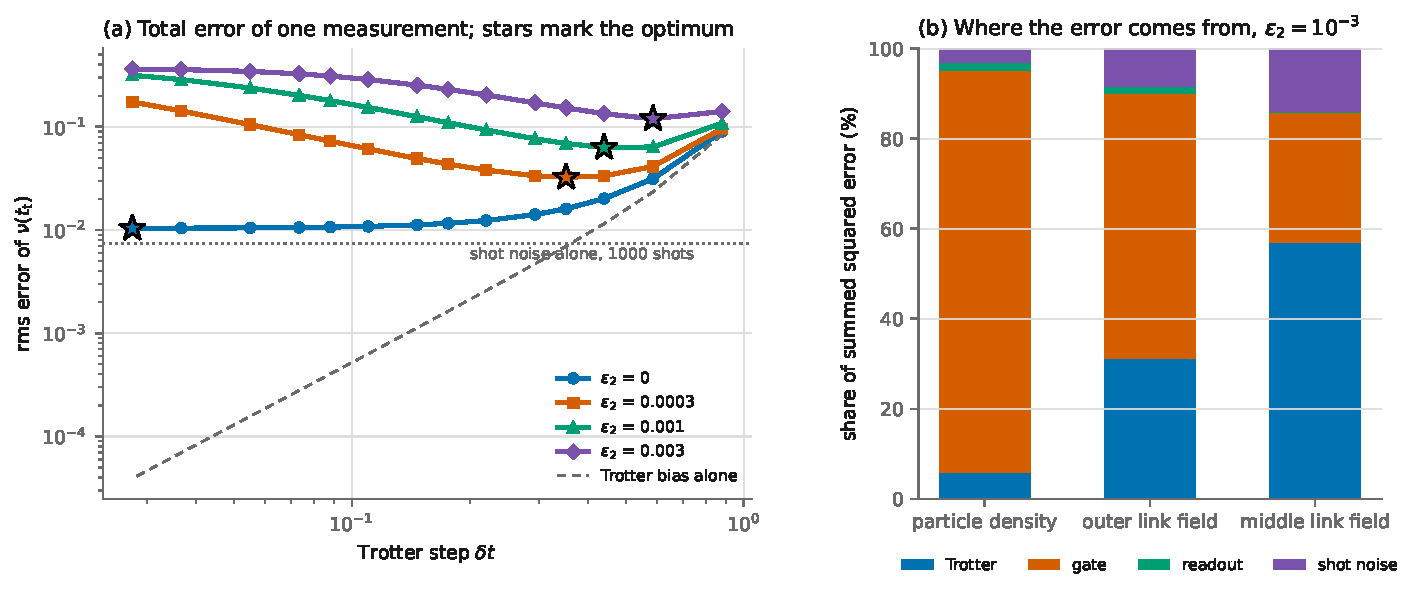
\includegraphics[width=\textwidth]{08_error_budget.pdf}
  \caption{(a) Root-mean-square error of a 1000-shot measurement of
  $\nu(t_{\mathrm{t}} = 1.76)$ against step size, with 1\,\% readout error, for
  four two-qubit error rates; stars mark the optimum. (b) Shares of the summed
  squared error at the optimum for $\epsilon_2 = 10^{-3}$. Produced by
  \texttt{scripts/08\_error\_budget.py}.}
  \label{fig:budget}
\end{figure}

\subsection{Ground state by SKQD}

At these parameters the ground state puts 71\,\% of its weight on the bare
vacuum $|0101\rangle$, 10\,\% on each of $|0110\rangle$ and $|1001\rangle$,
7.5\,\% on $|0011\rangle$, 1.7\,\% on $|1010\rangle$, and \num{6.5e-4} on
$|1100\rangle$, the configuration with the longest flux string. Confinement
suppresses exactly the bitstrings SKQD is most likely to miss.
Figure~\ref{fig:skqd} shows the exact expected SKQD energy error against the
number of shots per Krylov step. With four full Trotter steps of
$\delta t = 0.3$, the relative energy error falls below $10^{-3}$ at 12 shots
per step and below $10^{-6}$ at about 100. With a single hopping-only step, as
in Rosanowski \emph{et al.}, 50 shots are needed for $10^{-3}$. Gate error at
$\epsilon_2 = 3\times10^{-3}$ makes SKQD slightly worse, not better: 20 shots per
step instead of 12. Noise spreads probability over all sixteen bitstrings, but
the ten charged ones are discarded, so at a fixed shot count fewer samples land
in the neutral sector. At $N = 4$ the only error left in SKQD is coverage, and a
few hundred shots remove it.

\begin{figure}[t]
  \centering
  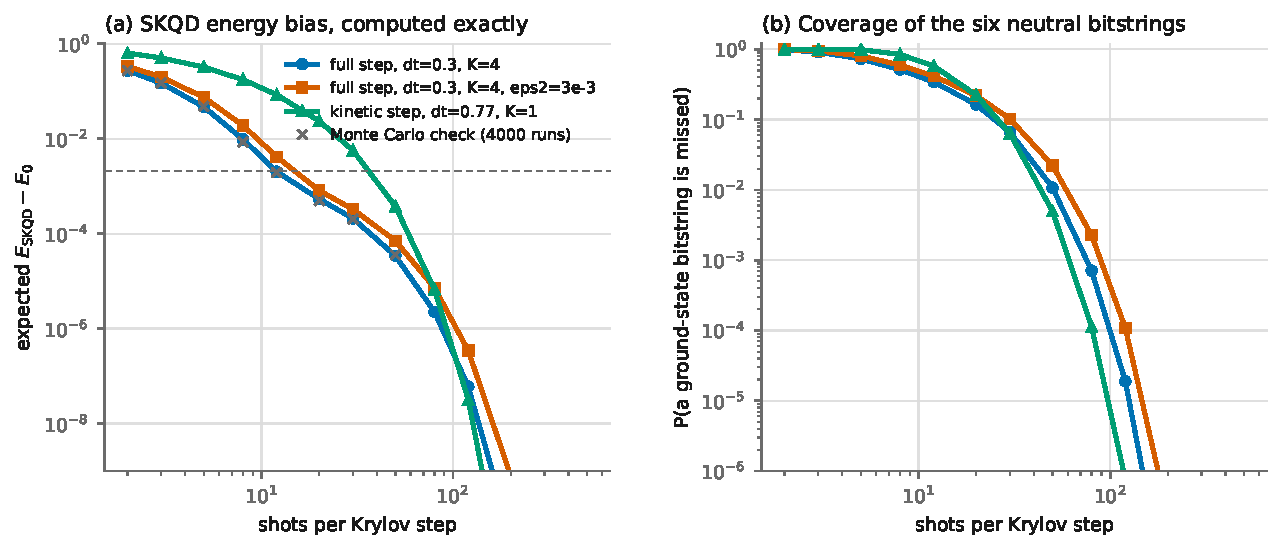
\includegraphics[width=0.9\textwidth]{07_skqd.pdf}
  \caption{(a) Exact expected SKQD energy error against shots per Krylov step,
  for four full second-order steps without and with gate error, and for one
  hopping-only step; crosses are a Monte Carlo check. The dashed line is a
  relative error of $10^{-3}$. (b) Probability that at least one bitstring of the
  ground state is never sampled. The single-step configuration uses a quarter of
  the total shots at the same horizontal position. Produced by
  \texttt{scripts/07\_skqd\_ground\_state.py}.}
  \label{fig:skqd}
\end{figure}

% ============================================================================
\section{Discussion}
\label{sec:discussion}
% ============================================================================

\todo{Due with the Results and Discussion draft. Three paragraphs planned:
(1) the depth rule $\epsilon^\ast n_{\mathrm{CX}} \approx 2$ against published
gate counts (Martinez: more than 200 gates; Farrell: 13,858 two-qubit gates) and
fidelities; (2) what the optimistic bias and the dephasing blind spot mean for
symmetry-based diagnostics in the literature (Martinez leakage, Nguyen symmetry
protection, Halimeh and Hauke); (3) limitations: depolarising and dephasing
models only, no coherent or correlated error, no amplitude damping, one
parameter point, $N = 4$, and a coarse lattice far from the continuum.}
